\documentclass{article}
%\usepackage[margin=1in]{geometry}
\usepackage{graphicx} % Required for inserting images
\usepackage{hyperref}
\usepackage{amsmath}
\usepackage{titling}
\usepackage{enumitem}
\usepackage{makecell}
\usepackage{minted}
 \usepackage{url}
\renewcommand\maketitlehooka{\null\mbox{}\vfill}
\renewcommand\maketitlehookd{\vfill\null}

\begin{document}
\centering

\title{\Huge Intro Deep Learning Homework 1}

\author{ \huge
Jaskin Kabir \\
\Large Student Id: 801186717 \\
\Large \href{https://github.com/jaskinkabir/Intro_Deep_Learning/tree/master/HM1}{GitHub:}\\\url{https://github.com/jaskinkabir/Intro_Deep_Learning/tree/master/HM1}
}

\date{January 2025}

\begin{titlingpage}
\maketitle
\end{titlingpage}

\section{Problem 1: Multilayer Perceptrons For Image Classification}

\begin{enumerate}[label=1\alph*. ]
    \item \textit{Three Hidden Layers}
    
    Using three hidden layers, consisting of 64, 32, and 16
    neurons respectively, the model was trained for 20
    epochs. As seen in the curves graphed in Figure
    \ref{fig:loss_1a}, the training loss curve has not yet
    begun to converge to the optimal solution after just 20
    epochs. To fully train the model, more epochs would be
    required. There is also significant overfit, as
    indicated by the gap between the training and validation
    accuracy curves.
    
    \begin{figure}[h]
        \centering
        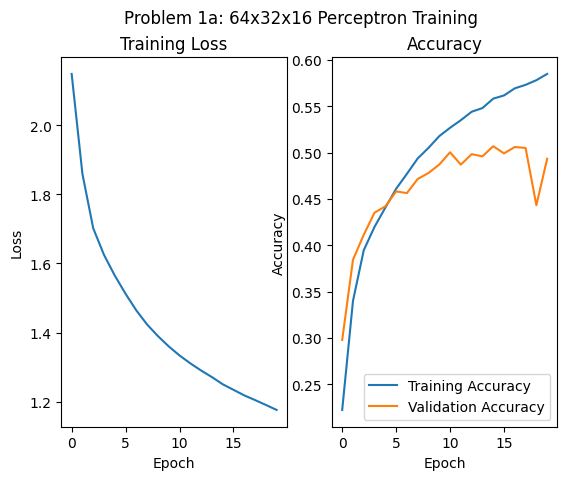
\includegraphics[width=0.5\textwidth]{images/loss_1a.png}
        \caption{Loss and Accuracy Curves for Three Hidden Layers}
        \label{fig:loss_1a}
    \end{figure} 
    The confusion matrix for this model can be seen in
    Figure \ref{fig:confusion_1a}.
    \begin{figure}[h]
        \centering
        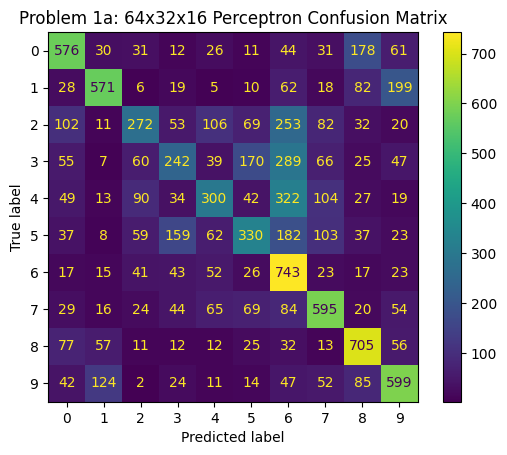
\includegraphics[width=0.5\textwidth]{images/conf_1a.png}
        \caption{Confusion Matrix for Three Hidden Layers}
        \label{fig:confusion_1a}
    \end{figure} 

    \newpage
    \item \textit{Five Hidden Layers}
    
    Using five hidden layers, consisting of 256, 128, 64,
    32, and 16 neurons respectively, the model was trained
    for 20 epochs. As seen in the curves graphed in Figure
    \ref{fig:loss_1b}, the model has not yet converged to
    the optimal solution after 20 epochs. There is also
    significant overfit, but not as pronounced as it is in
    the three hidden layer model.
    \begin{figure}[h]
        \centering
        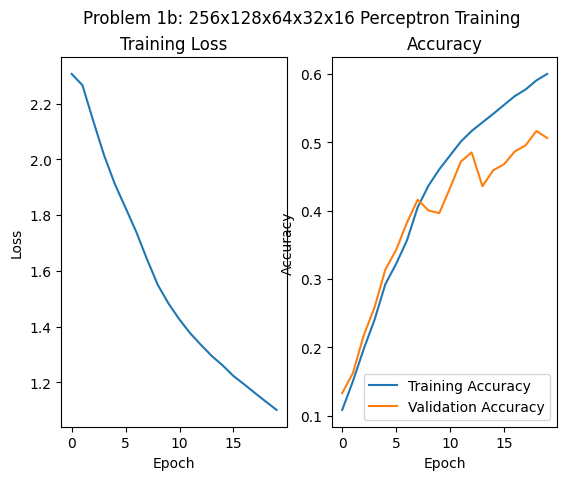
\includegraphics[width=0.5\textwidth]{images/loss_1b.png}
        \caption{Loss and Accuracy Curves for Five Hidden Layers}
        \label{fig:loss_1b}
    \end{figure}
    The confusion matrix for this model can be seen in
    Figure \ref{fig:confusion_1b}.
    \begin{figure}[h]
        \centering
        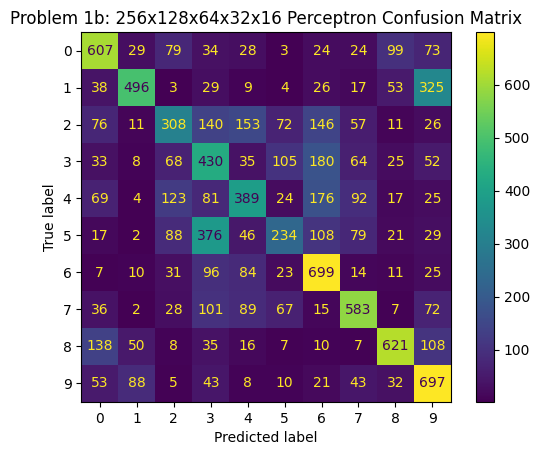
\includegraphics[width=0.5\textwidth]{images/conf_1b.png}
        \caption{Confusion Matrix for Five Hidden Layers}
        \label{fig:confusion_1b}
    \end{figure} 

\textbf{Comparison}

Table \ref{tab:comparison1} shows that the more complex
model performed better in every metric. However, even the
5-layer model was barely more accurate than a coin toss. The
models are likely underfit, as they have not yet converged
to the optimal solution. Additionally, the multilayer
perceptron is not the ideal paradigm for image
classification. A convolutional neural network would likely
outperform both of these models.
\begin{table}[h]
    \centering
    \begin{tabular}{|c|c|c|c|}
        \hline
        \textbf{Metric (\%)} & \textbf{3-Layer Model} &
        \textbf{5-Layer Model} & \textbf{$\Delta$} \\
        \hline
        Accuracy & 49.3 & 50.6 & 2.59 \\
        Precision & 49.8 & 51.6 & 3.37 \\
        Recall & 49.3 & 50.6 & 2.59 \\ 
        F1 Score & 48.2 & 50.1 & 3.69 \\
        \hline
    \end{tabular}
    \caption{Comparison of Evaluation Metrics}
    \label{tab:comparison1}
\end{table}
\end{enumerate}

\section{Problem 2: Housing Price Regression}
\begin{enumerate}[label=1\alph*. ]
    \item \textit{Perceptron Regressor}
    
    The housing dataset has several categorical features. In
    order to use this data to train the model, the categorical values like
    'yes' or 'no' were converted to 1 and 0 repsectively. Using 2 layers,
    woth 64 and 32 neurons respectively, the model was trained for 500 epochs.
    As seen in the curves graphed in Figure \ref{fig:loss_2a}, the model has
    \begin{figure}[h]
        \centering
        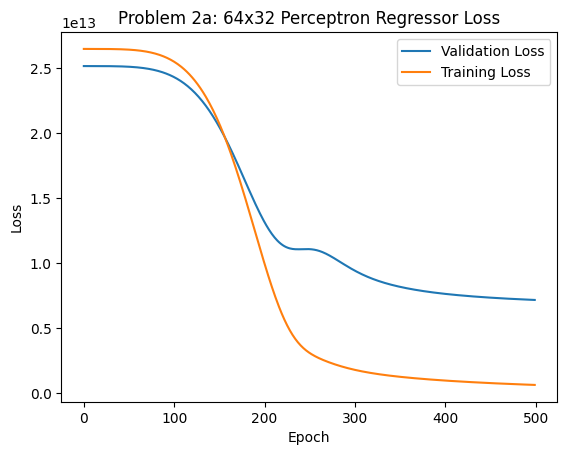
\includegraphics[width=0.5\textwidth]{images/loss_2a.png}
        \caption{Loss and Accuracy Curves for Perceptron Regressor}
        \label{fig:loss_2a}
    \end{figure}


\end{enumerate}

\end{document}